%% Fall 2013 MDM Homework Template
\documentclass[12pt,letterpaper]{article}

\usepackage[utf8]{inputenc}
\usepackage[T1]{fontenc}
\usepackage{amsmath}
\usepackage{amsfonts}
\usepackage{amssymb}
\usepackage{amsthm}
\usepackage[left=2cm,right=2cm,top=2cm,bottom=2cm,headheight=22pt]{geometry}
\usepackage{fancyhdr}
\usepackage{setspace}
\usepackage{lastpage}
\usepackage{graphicx}


\theoremstyle{definition}
\newtheorem{task}{Task}

\begin{document}

%other parameters
\setlength{\parskip}{1ex plus 0.5ex minus 0.2ex}
\setlength{\parindent}{0pt}

%header and footer parameters
\pagestyle{fancy}
\lhead{Math 1100}
\chead{Weekly Homework}
\rhead{Due: January 29}
\lfoot{}
\cfoot{\emph{Prof. Hitchman}}
\rfoot{}



\begin{center}
{
\Large
\textbf{Knots: Written Assignment \#3}
}
\end{center}

To earn a passing mark, your assignment must:
\begin{itemize}
\item be written legibly. Diagrams may be hand drawn, but should be clear enough to read easily.
\item address the writing prompts below.
\item conform to reasonable standards for grammar, spelling, and usage of the English language with minimal errors. (You may consider seeking help on writing from the Writing Center in the Academic Learning Center. http://www.uni.edu/unialc/writing-center)
\item be turned in by 3pm on Friday, January 29.
\end{itemize}

\begin{task}
Draw planar projections of (1) a trefoil knot and (2) a figure eight knot. Make them look nice and label which one is which.
\end{task}

\begin{task}
Draw a planar projection of the unknot which happens to have six crossings. (You might make one up by using 
Reidemeister moves to \emph{complicate} things, rather than to simplify.) Be sure to make a pretty picture. 

Explain how you know your knot is the same as the unknot. 
\end{task}


\begin{task}
We have seen the following knot before, and noted that it is a planar projection of an unknot.
Show that this knot is equivalent to the unknot be describing a sequence of Reidemeister moves which change this planar projection into an ordinary circle.

Draw pictures of the steps along the way, and clearly label each transition with the type of Reidemeister move made.
\end{task}

\begin{figure}[h]
    \centering
    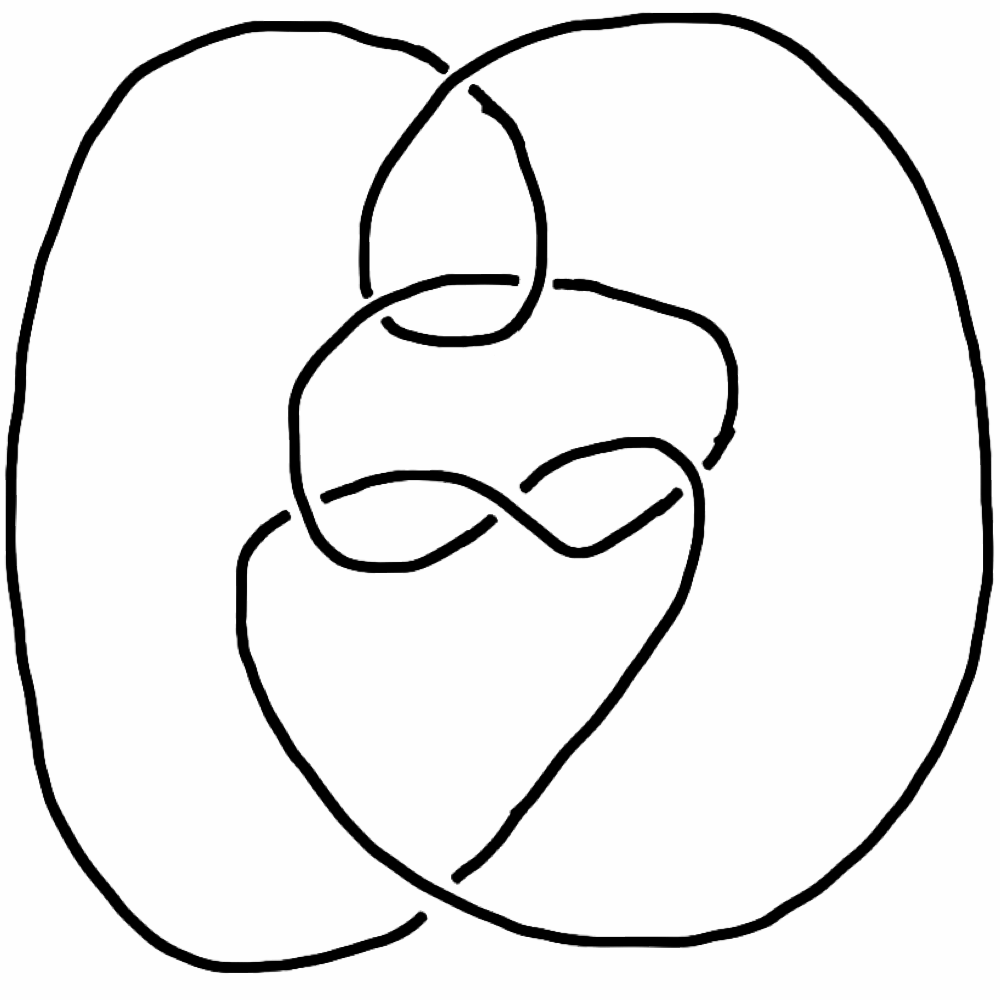
\includegraphics[width=.5\textwidth]{knotpics/9SeptQ5b.png}
    \caption{An Unknot}
\end{figure}


\end{document}
%sagemathcloud={"zoom_width":100}